\section{Modalità di esecuzione dei test}
In questa sezione si andrà ad analizzare le performance delle tre soluzioni VPN descritte nei capitoli precedenti, al fine di valutare quale di esse offre le prestazioni migliori.
Le prestazioni verranno valutate analizzando il throughput, la sua stabilità e la percentuale di packetloss.
I software che sono stati utilizzati per effettuare le misurazioni questi dati sono \texttt{iPerf3} e \texttt{mrt}.

\subsection{Panoramica di \texttt{iPerf3}}
\texttt{iPerf} è uno strumento open source che permette di misurare le prestazioni di una rete.
Per effettuare le misurazioni, iPerf crea dei flussi di dati su TCP, UDP o SCTP e invia traffico da un host all'altro; al termine del trasferimento, oltre a un report dettagliato in base al tipo di misurazione richiesta, mostra la larghezza di banda media disponibile.
In questo modo, gli utenti possono determinare il throughput effettivamente utilizzabile.

\begin{figure}[ht]
    \centering
    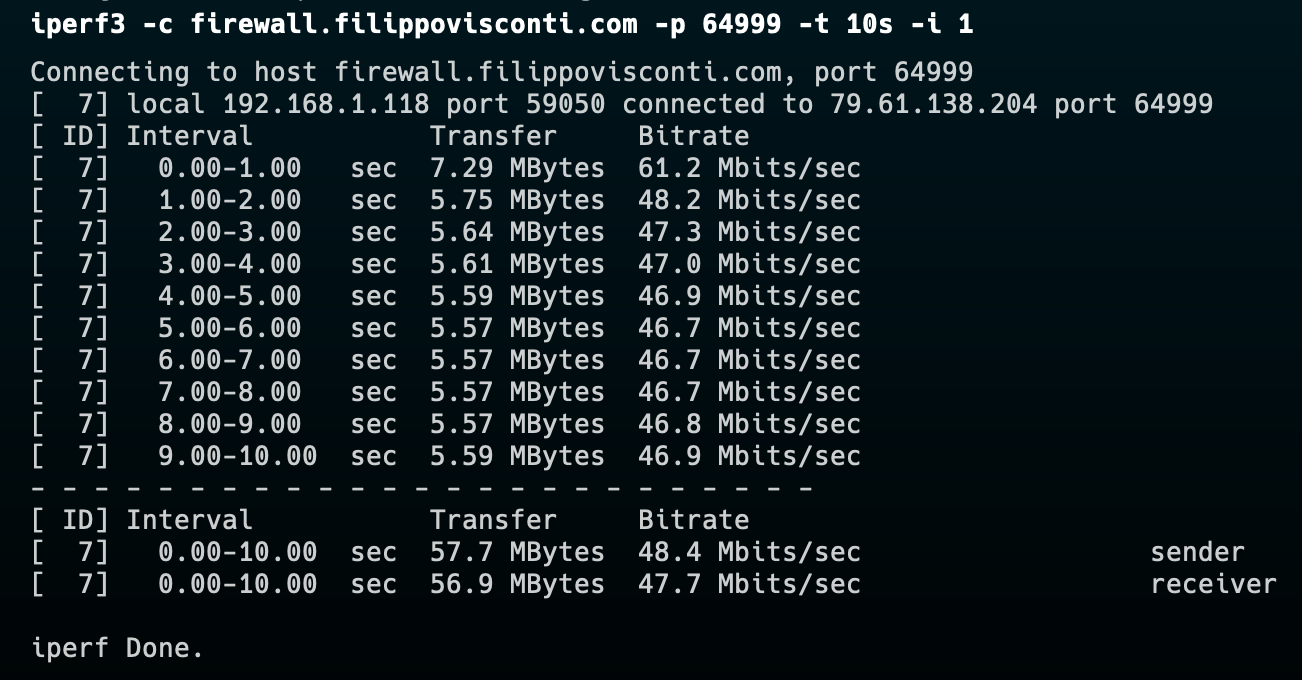
\includegraphics[width=10cm]{figure/iperfSample.png}
    \caption{Esempio di output di iPerf3}
\end{figure}

\subsection{Panoramica di \texttt{mrt}}
\texttt{mtr} è un altro software di misurazione delle performance di una rete, che sostanzialmente unisce i risultati di traceroute e ping.
I test effettuati da mtr sono unidirezionali, dunque è opportuno effettuare misurazioni manualmente in entrambe le direzioni, in quanto i risultati differire in maniera sostanziale. Per avere una misurazione affidabile, è consigliabile far durare il test almeno 10 minuti.

\begin{figure}[ht]
    \centering
    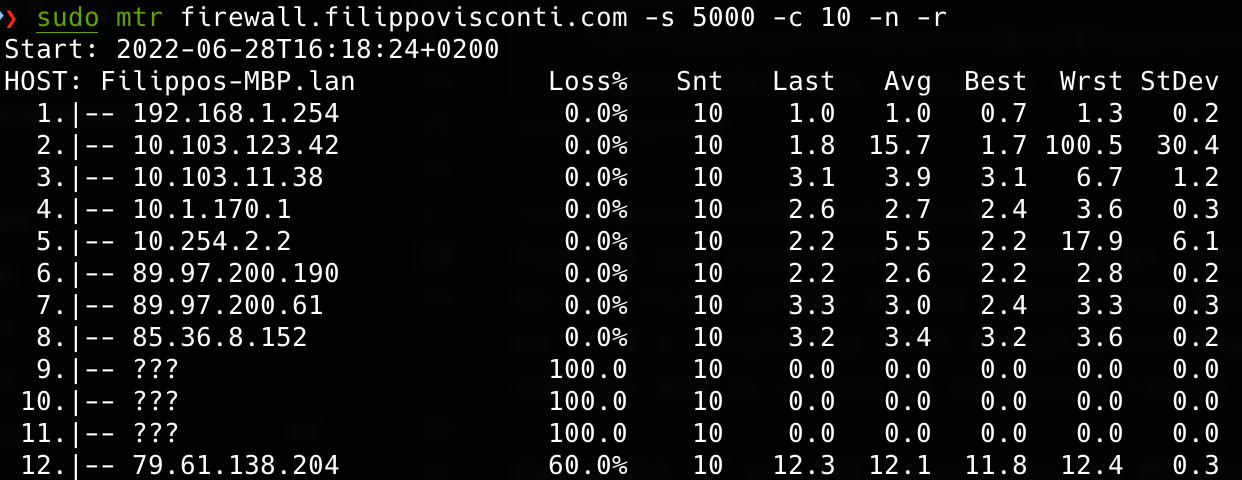
\includegraphics[width=10cm]{figure/mtrSample.png}
    \caption{Esempio di output di mrt}
\end{figure}

\subsubsection{Spiegazione del formato dell'output}
Nella prima colonna, si legge un numero e un indirizzo IP: il numero corrisponde alla distanza in hop tra l'host da cui parte il test e l'IP indicato alla sua destra.
La seconda colonna, \texttt{Loss\%}, indica la percentuale di pacchetti che quell'IP ha perso. È auspicabile un valore inferiore all'1\% per una connessione affidabile.
La terza colonna, \texttt{Snt}, indica il numero di pacchetti inviati a quell'IP.
Le successive 4 colonne indicano il valore dell'ultimo, del medio, del migliore e del peggiore round-trip-time in millisencondi - ossia il tempo necessario affinché un pacchetto parta dal mittente, raggiunga il destinatario, e torni indietro.
L'ultima colonna indica la deviazione standard tra questi ultimi 4 valori.
I valori dalla terza colonna in poi forniscono dunque informazioni sulla latenza della rete. È desiderabile il valore più basso possibile. Tuttavia,  spesso la latenza dipende da fattori esterni alla rete locale.

Nella misurazione di esempio, è stato richiesto l'invio di 10 pacchetti (\texttt{-c 10}) di dimensione 5000 byte (\texttt{-s 5000}).
Per gli hop 9, 10 e 11, si ha un risultato anomalo: nessun IP restituito e 100\% di packet loss.
Questo risultato non mostra problemi di connessione, ma indica semplicemente che l'host non ha risposto alle richieste indirizzate a lui (per i motivi più disparati, da un carico di lavoro troppo altro, a un firewall che fa cadere quel tipo di pacchetto), e che però, visto che l'hop 12 risponde correttamente, ha inoltrato correttamente quelle destinate a chi gli succede.



\subsection{Scelta della configurazione di test}
Ancora del testo

\subsection{Criteri di valutazione}
Per dare una valutazione complessiva alle tre soluzioni testate, si andranno a tenere in considerazione i seguenti parametri: throughput, percentuale di packet loss per un pacchetto di grandi dimensioni e latenza media.

\subsubsection{Throughput}
Il throughput di un canale di comunicazione misura la quantità di dati che può essere trasferita tra mittente e destinatario in una data unità di tempo. In ambito reti, si è soliti utilizzare come unità di tempo il secondo e come quantità di dati il bit, o suoi multipli (Kbit, Mbit, Gbit).
La velocità e l'affidabilità di trasmissione dei pacchetti sono parametri fondamentali ed è necessario che siano in grado di soddisfare le necessità dell'azienda proprietaria della rete. Packet loss, latenza e jitter influenzano il throughput di una rete, e più sono elevati, più le performance degradano. Minimizzare tutti questi fattori è un punto cardine della progettazione e ottimizzazione di una rete.
La larghezza di banda potrebbe essere confusa con il throughput; è un valore che misura sempre una quantità di bit trasferiti in un'unità di tempo, ma misura il limite massimo teorico, e non quello reale.

È importante sottolineare che una larghezza di banda maggiore non conferisce più velocità, bensì dà soltanto la possibilità di trasferire allo stesso momento una quantità di dati maggiore. Se si hanno problemi di latenza e di perdita dei pacchetti, questi non verranno risolti aumentando la larghezza di banda.


\subsubsection{Packetloss}
Quando un pacchetto non riesce a raggiungere la destinazione prevista, si verifica il fenomeno della perdita di pacchetti, packet loss.
Un utente avverte questo problema come interruzioni della rete, perdita di connettività e una velocità di connessione rallentata.
Le situazioni in cui si soffre maggiormente questo problema sono tutte quelle in cui è richiesta elaborazione di dati in real-time, dove i ritardi non sono tollerati.

The Transmission Control Protocol (TCP) detects packet loss and performs retransmissions to ensure reliable messaging. Packet loss in a TCP connection is also used to avoid congestion and thus produces an intentionally reduced throughput for the connection.

In real-time applications like streaming media or online games, packet loss can affect a user's quality of experience (QoE).
Causes[edit]
The Internet Protocol (IP) is designed according to the end-to-end principle as a best-effort delivery service, with the intention of keeping the logic routers must implement, as simple as possible. If the network made reliable delivery guarantees on its own, that would require store and forward infrastructure, where each router devotes a significant amount of storage space to packets while it waits to verify that the next node properly received them. A reliable network would not be able to maintain its delivery guarantees in the event of a router failure. Reliability is also not needed for all applications. For example, with live streaming media, it is more important to deliver recent packets quickly than to ensure that stale packets are eventually delivered. An application or user may also decide to retry an operation that is taking a long time, in which case another set of packets will be added to the burden of delivering the original set. Such a network might also need a command and control protocol for congestion management, adding even more complexity.

To avoid all of these problems, the Internet Protocol allows for routers to simply drop packets if the router or a network segment is too busy to deliver the data in a timely fashion. This is not ideal for speedy and efficient transmission of data, and is not expected to happen in an uncongested network.[4] Dropping of packets acts as an implicit signal that the network is congested, and may cause senders to reduce the amount of bandwidth consumed, or attempt to find another path. For example, using perceived packet loss as feedback to discover congestion, the Transmission Control Protocol (TCP) is designed so that excessive packet loss will cause the sender to throttle back and stop flooding the bottleneck point with data.

Packets may also be dropped if the IPv4 header checksum or the Ethernet frame check sequence indicates the packet has been corrupted. Packet loss can also be caused by a packet drop attack.

Measurement[edit]
Packet loss may be measured as frame loss rate defined as the percentage of frames that should have been forwarded by a network but were not.[8]

Acceptable packet loss[edit]
Packet loss is closely associated with quality of service considerations. The amount of packet loss that is acceptable depends on the type of data being sent. For example, for voice over IP traffic, one commentator reckoned that "[m]issing one or two packets every now and then will not affect the quality of the conversation. Losses between 5% and 10% of the total packet stream will affect the quality significantly."[9] Another described less than 1% packet loss as "good" for streaming audio or video, and 1–2.5% as "acceptable".[10]

\subsubsection{Latenza}
Network latency:

The latency data is shown in the last five columns of the report (the second column shows the progressive number of the ICMP packets sent). Normally the latency increases proportionally to the test execution time. If the growth is proportional and does not present significant jumps, this means that there are no problems on the network. They do not indicate anomalies nor peak values on the single node 6.

Conversely, if from node 8 onwards high latency values are found (compared to the first 6 hops), which persist until the last hops, it could indicate the presence of numerous problems on the network, such as inadequate configurations of network cards or routers, abnormally working services or network congestion.


\section{Misure senza VPN}
\begin{figure}[ht]
    \centering
    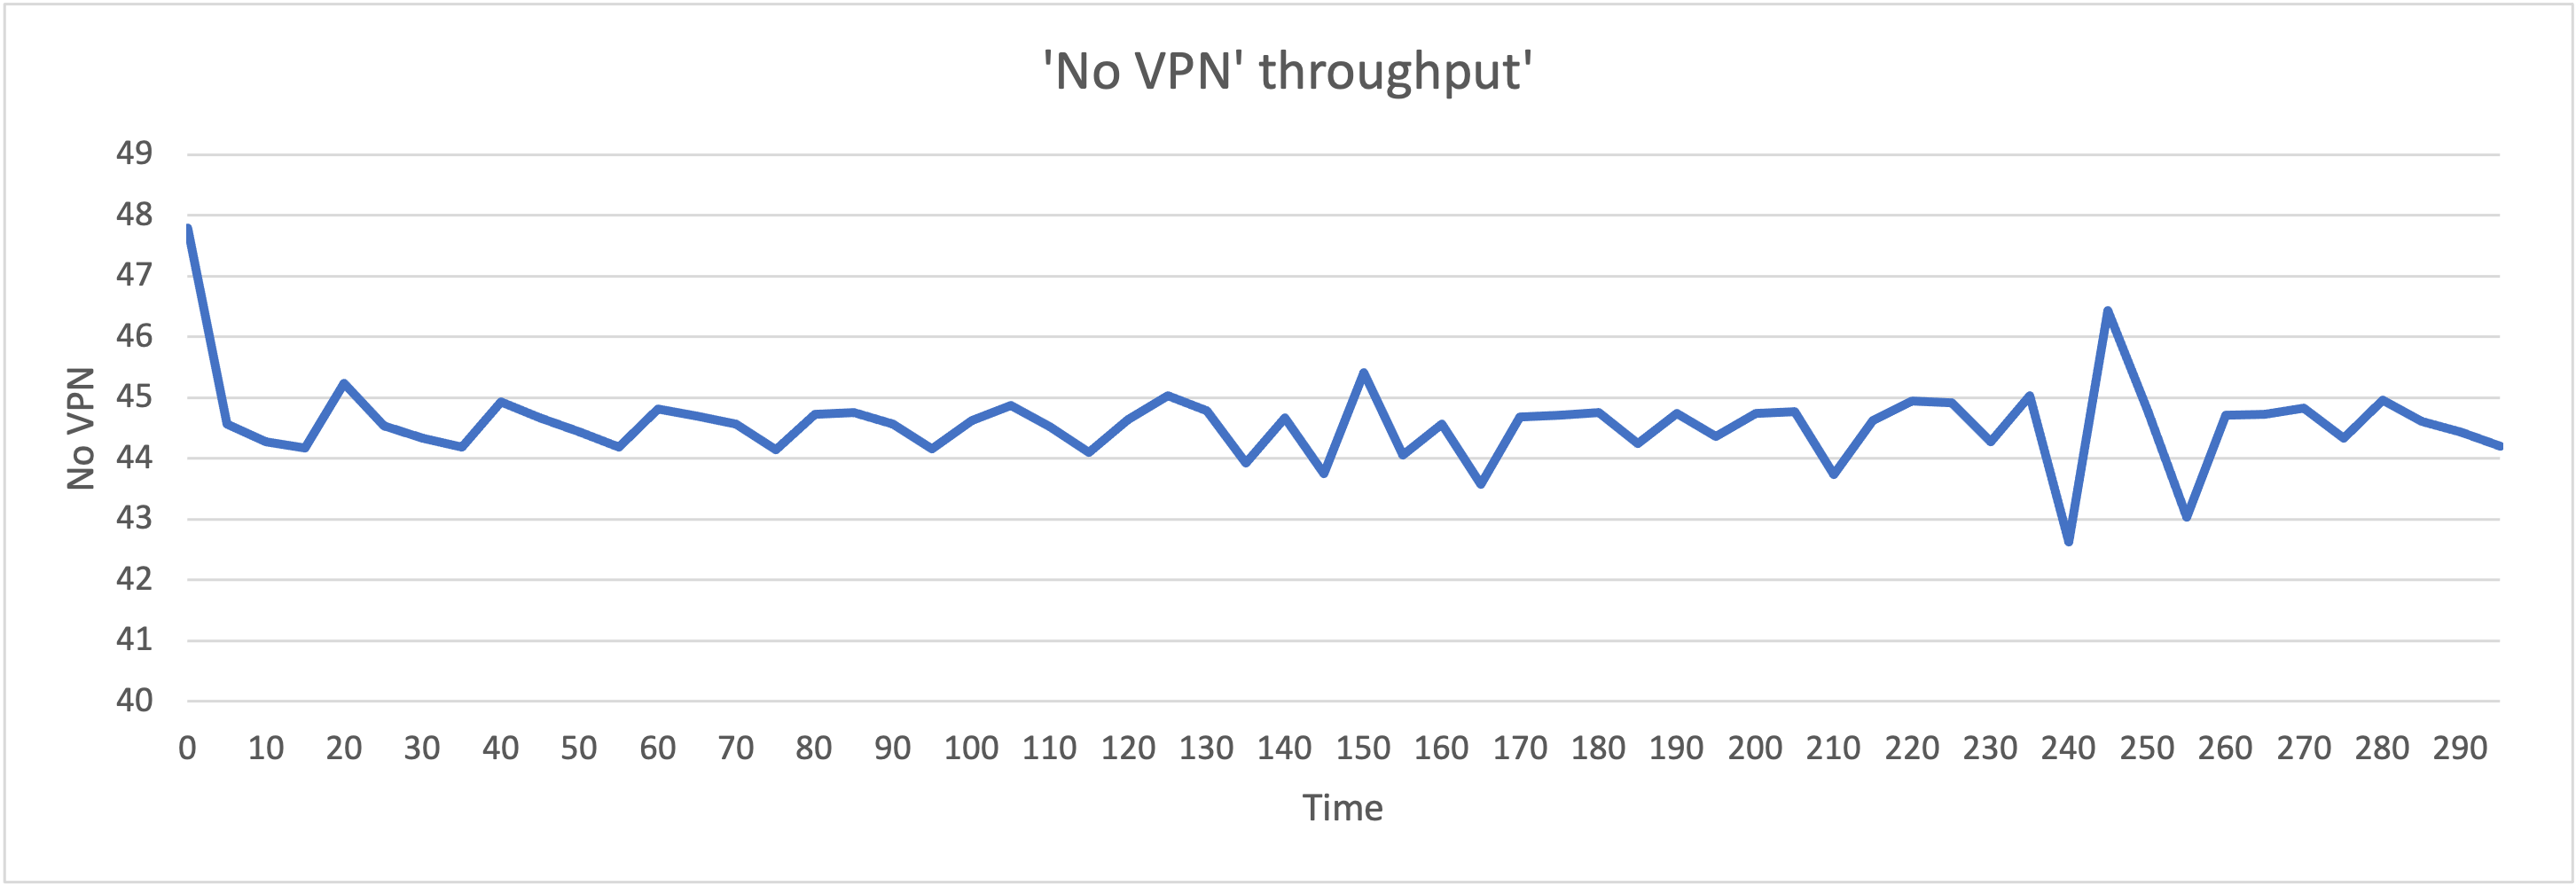
\includegraphics[width=12cm]{figure/vpn_thr.png-1.png}
    \caption{Throughput senza VPN su 300 secondi}
\end{figure}


\section{Misure con IPSec e IKEv2}
\begin{figure}[ht]
    \centering
    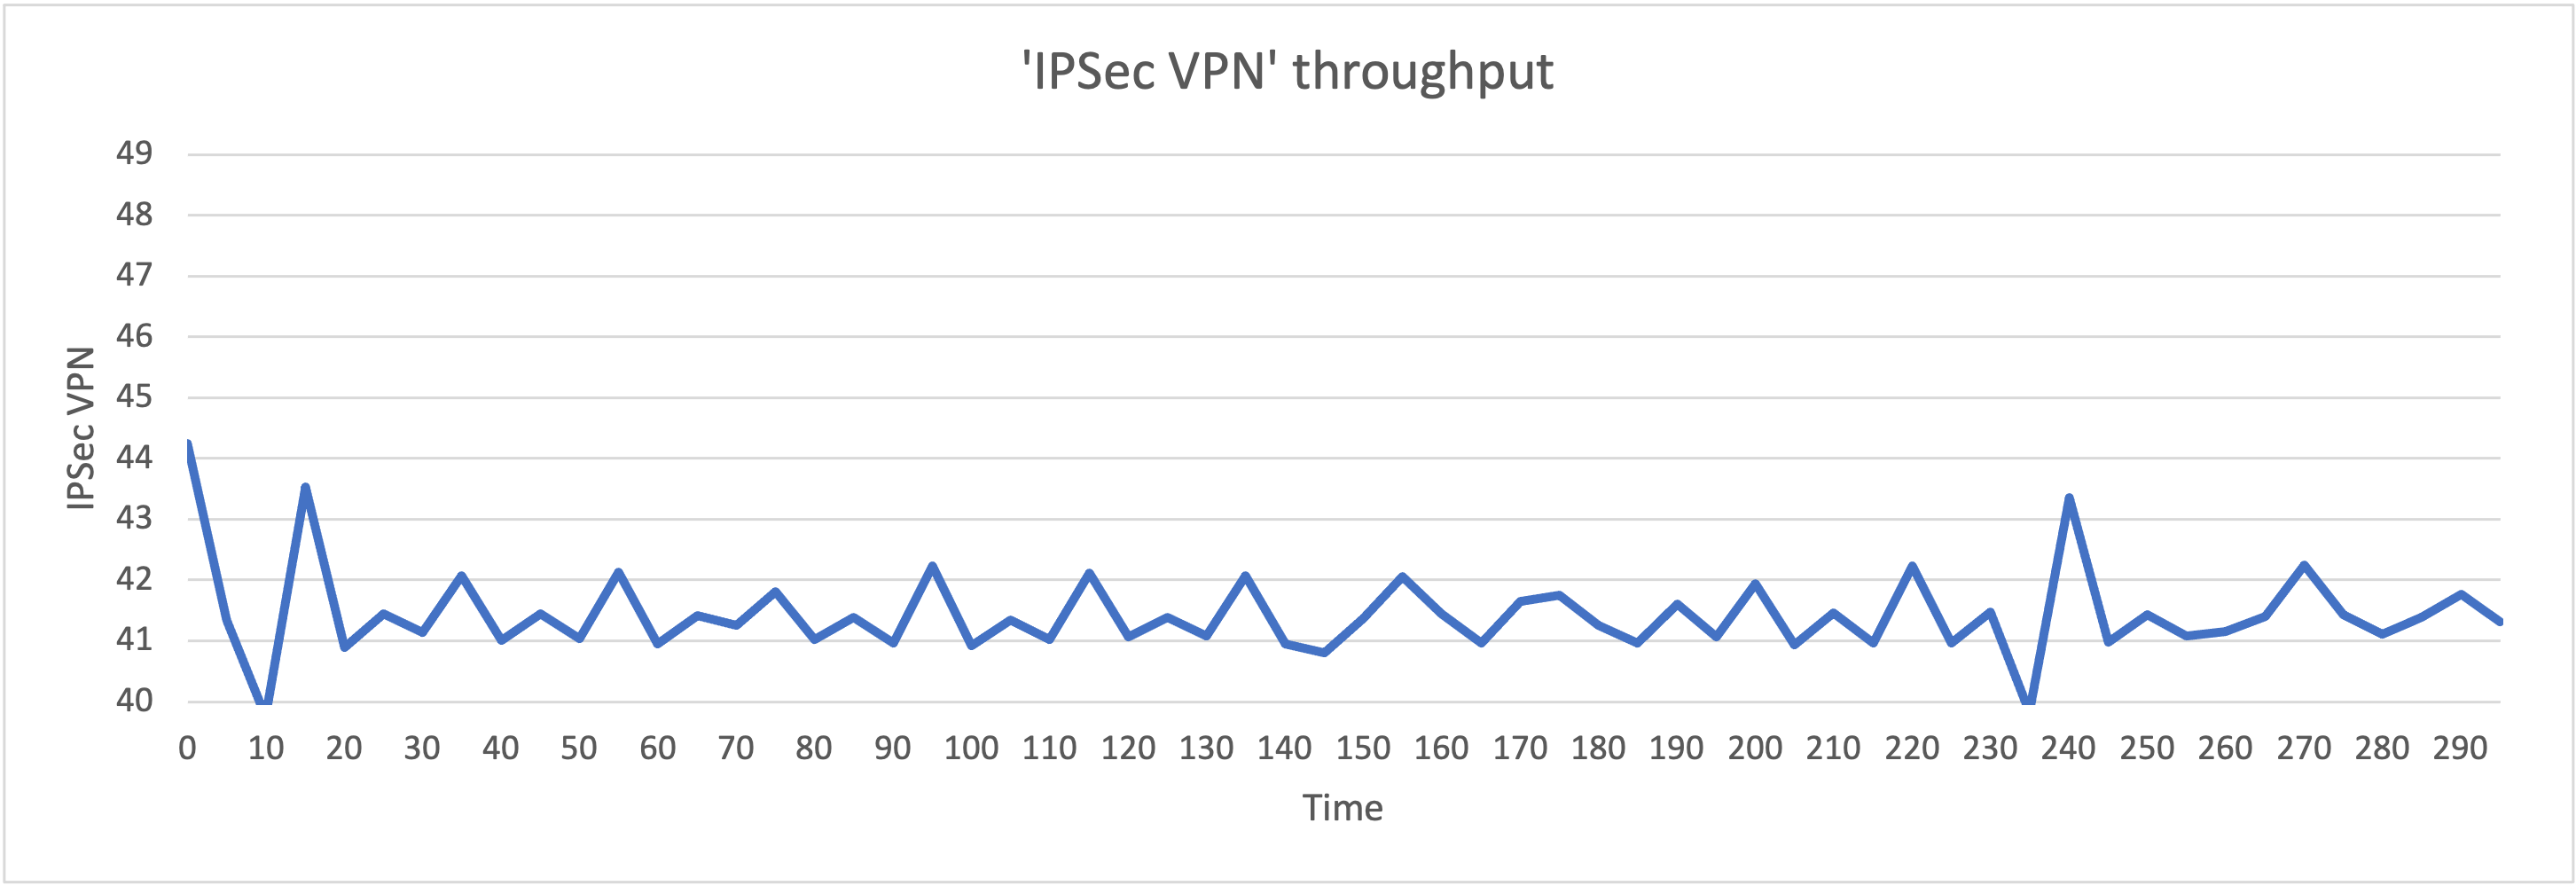
\includegraphics[width=12cm]{figure/vpn_thr.png-2.png}
    \caption{IPSec Throughput su 300 secondi}
\end{figure}

\section{Misure con OpenVPN over TCP}
\begin{figure}[ht]
    \centering
    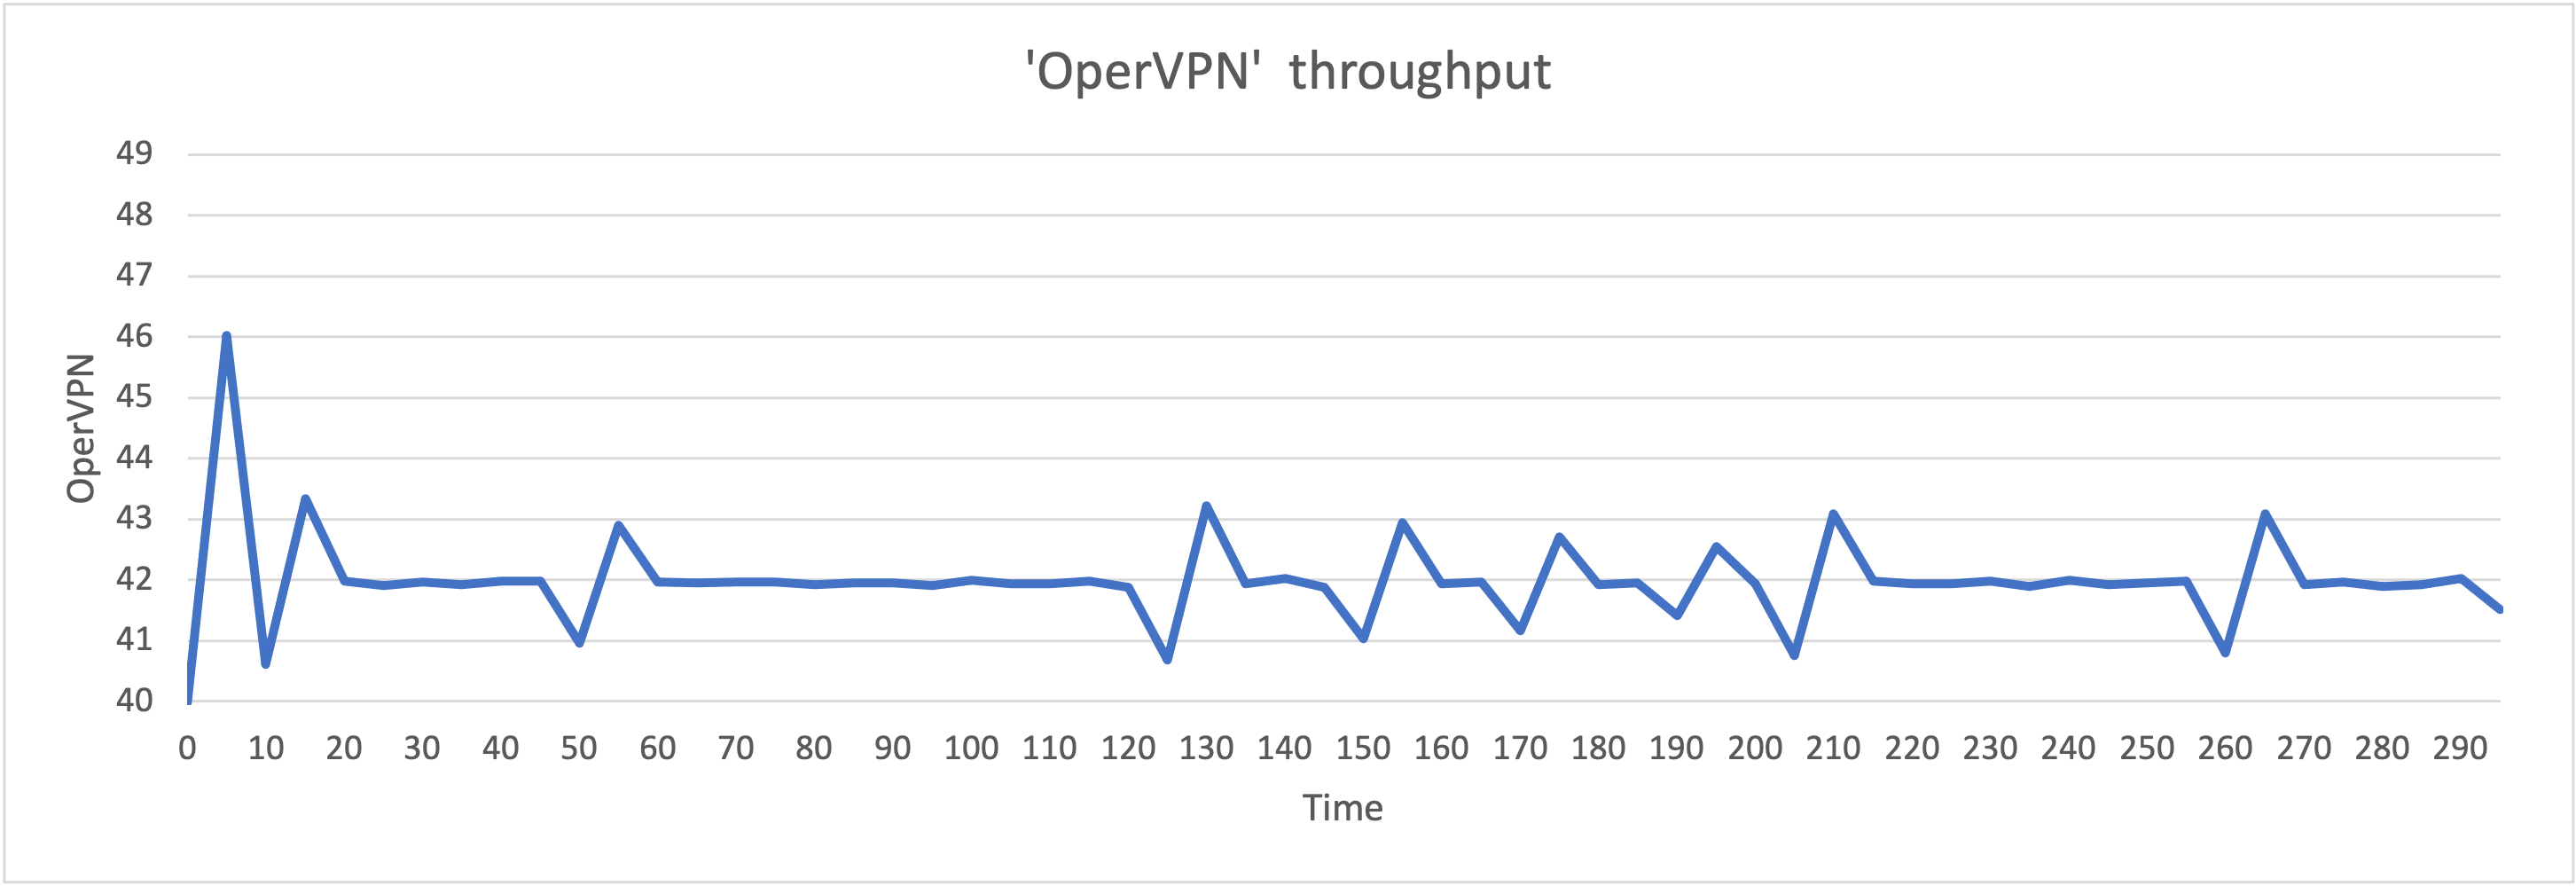
\includegraphics[width=12cm]{figure/vpn_thr.png-3.png}
    \caption{OpenVPN Throughput su 300 secondi}
\end{figure}

\section{Misure con WireGuard}
\begin{figure}[ht]
    \centering
    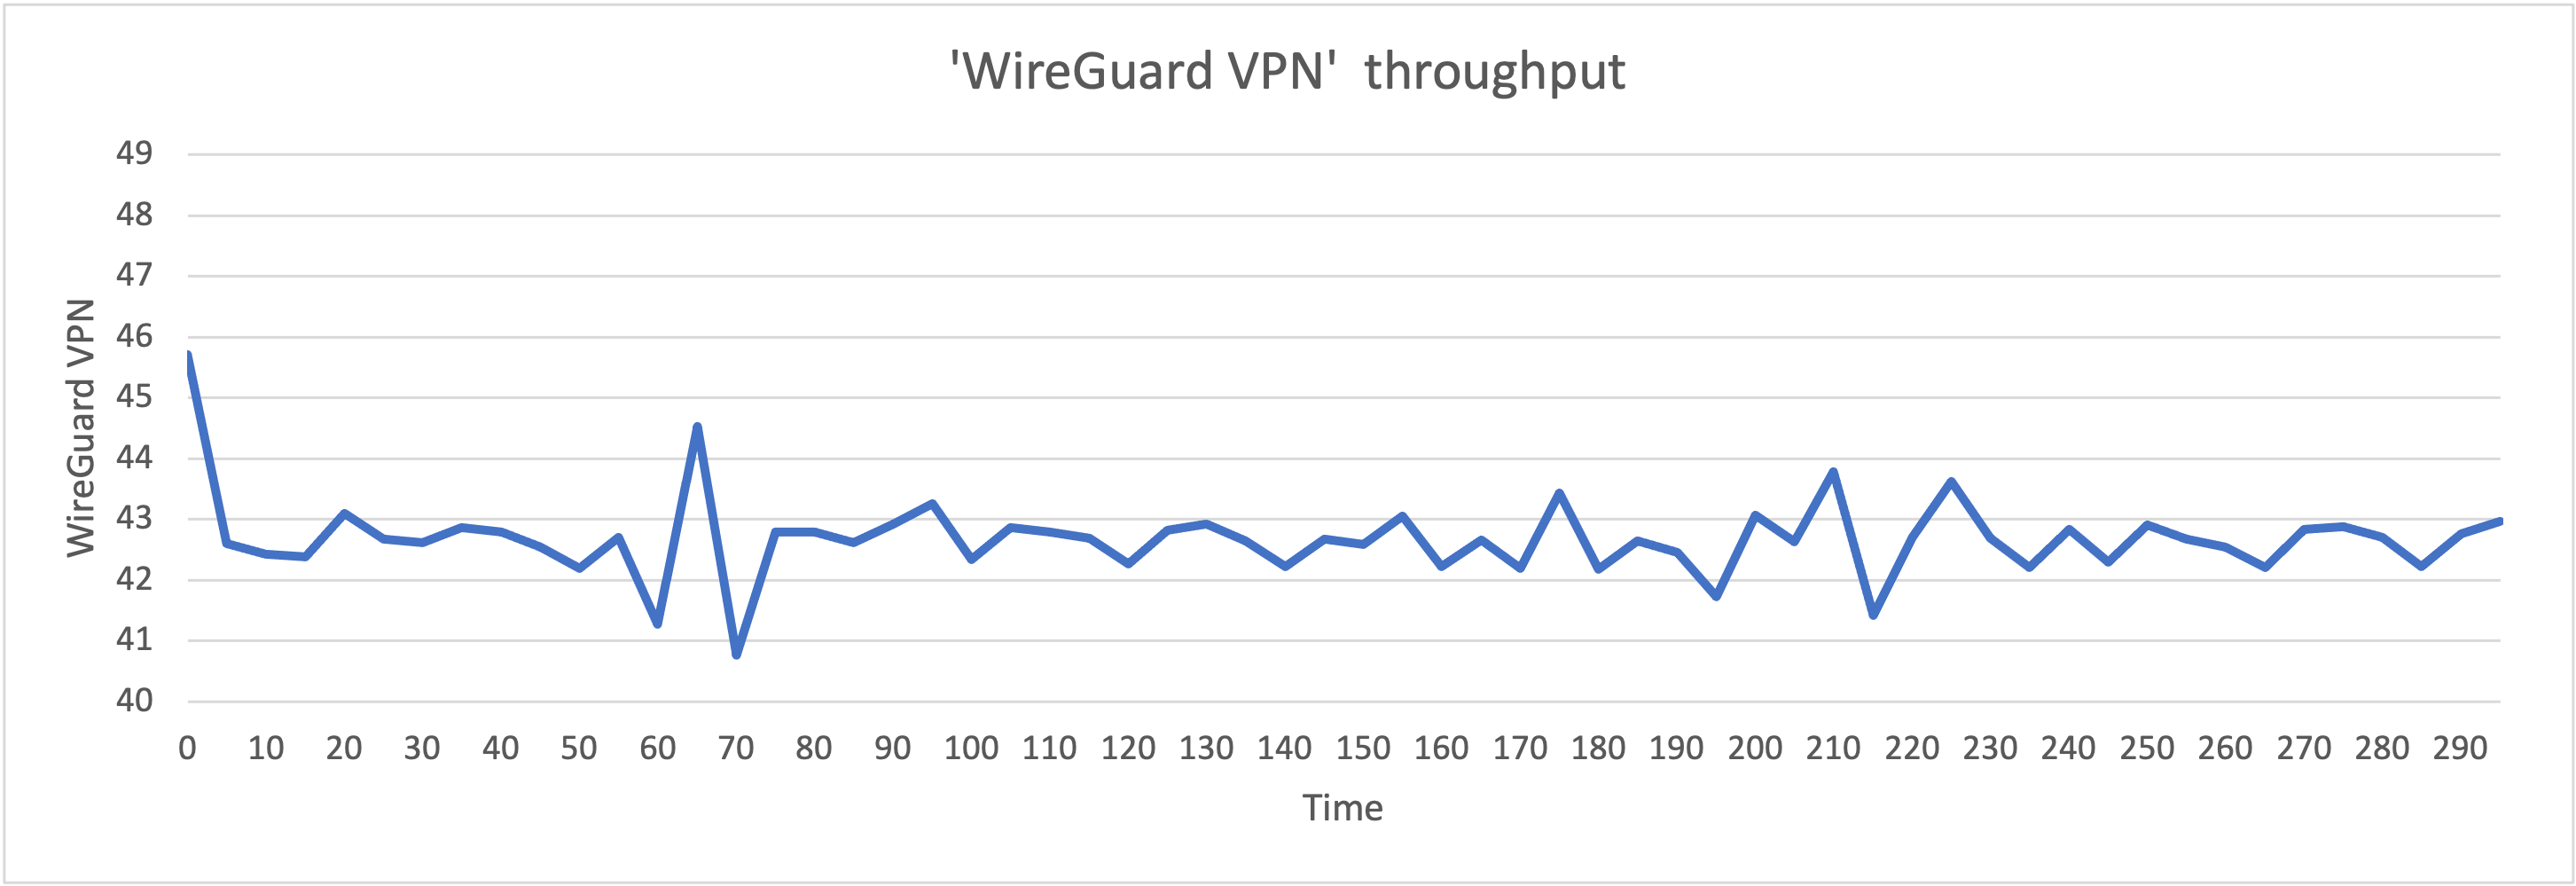
\includegraphics[width=12cm]{figure/vpn_thr.png-4.png}
    \caption{WireGuard Throughput su 300 secondi}
\end{figure}

\section{Analisi delle misure}
\begin{figure}[ht]
    \centering
    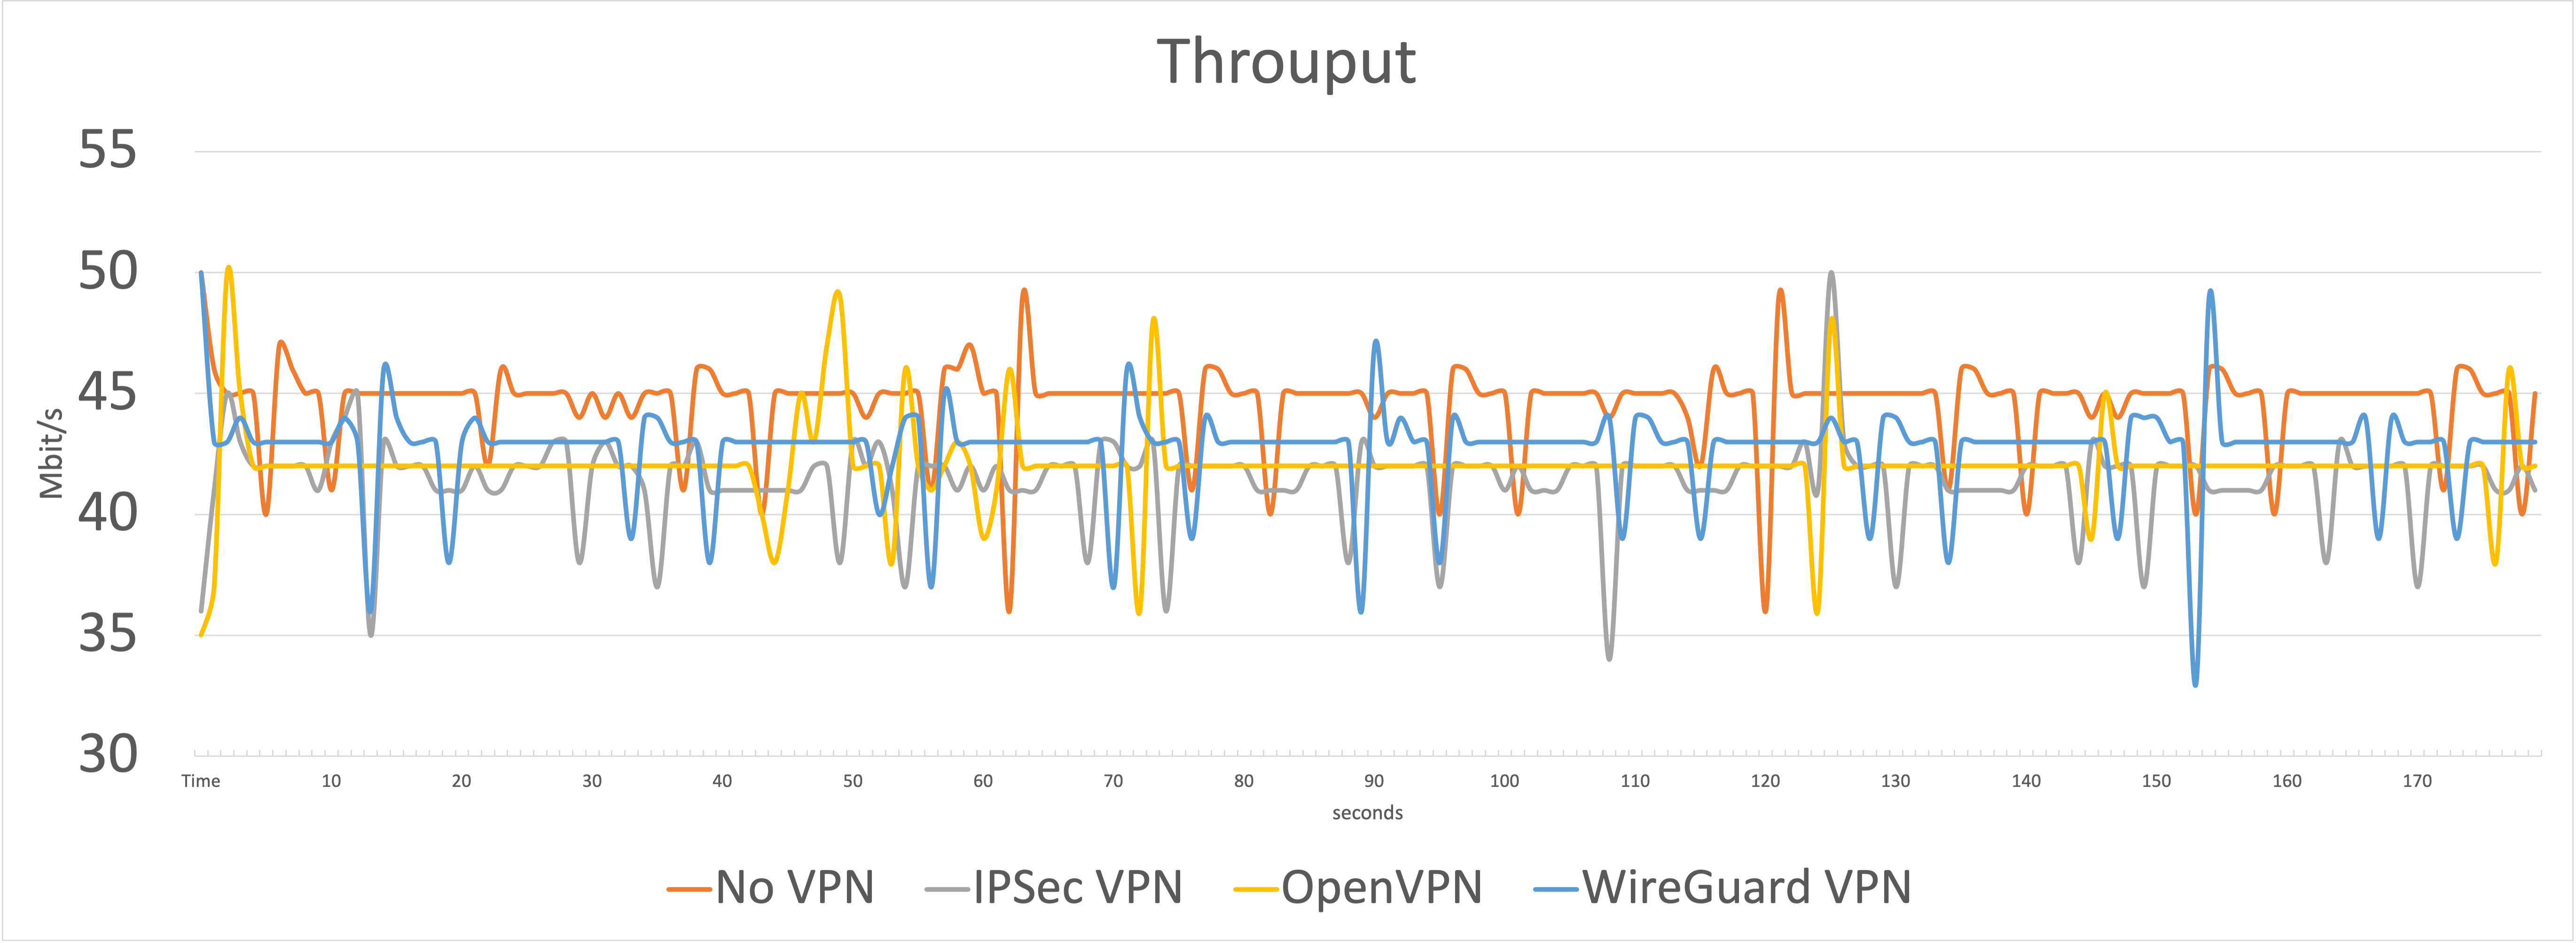
\includegraphics[width=14cm]{figure/rawThroughput.png}
    \caption{Confronto dei throughput grezzi}
\end{figure}

\begin{figure}[ht]
    \centering
    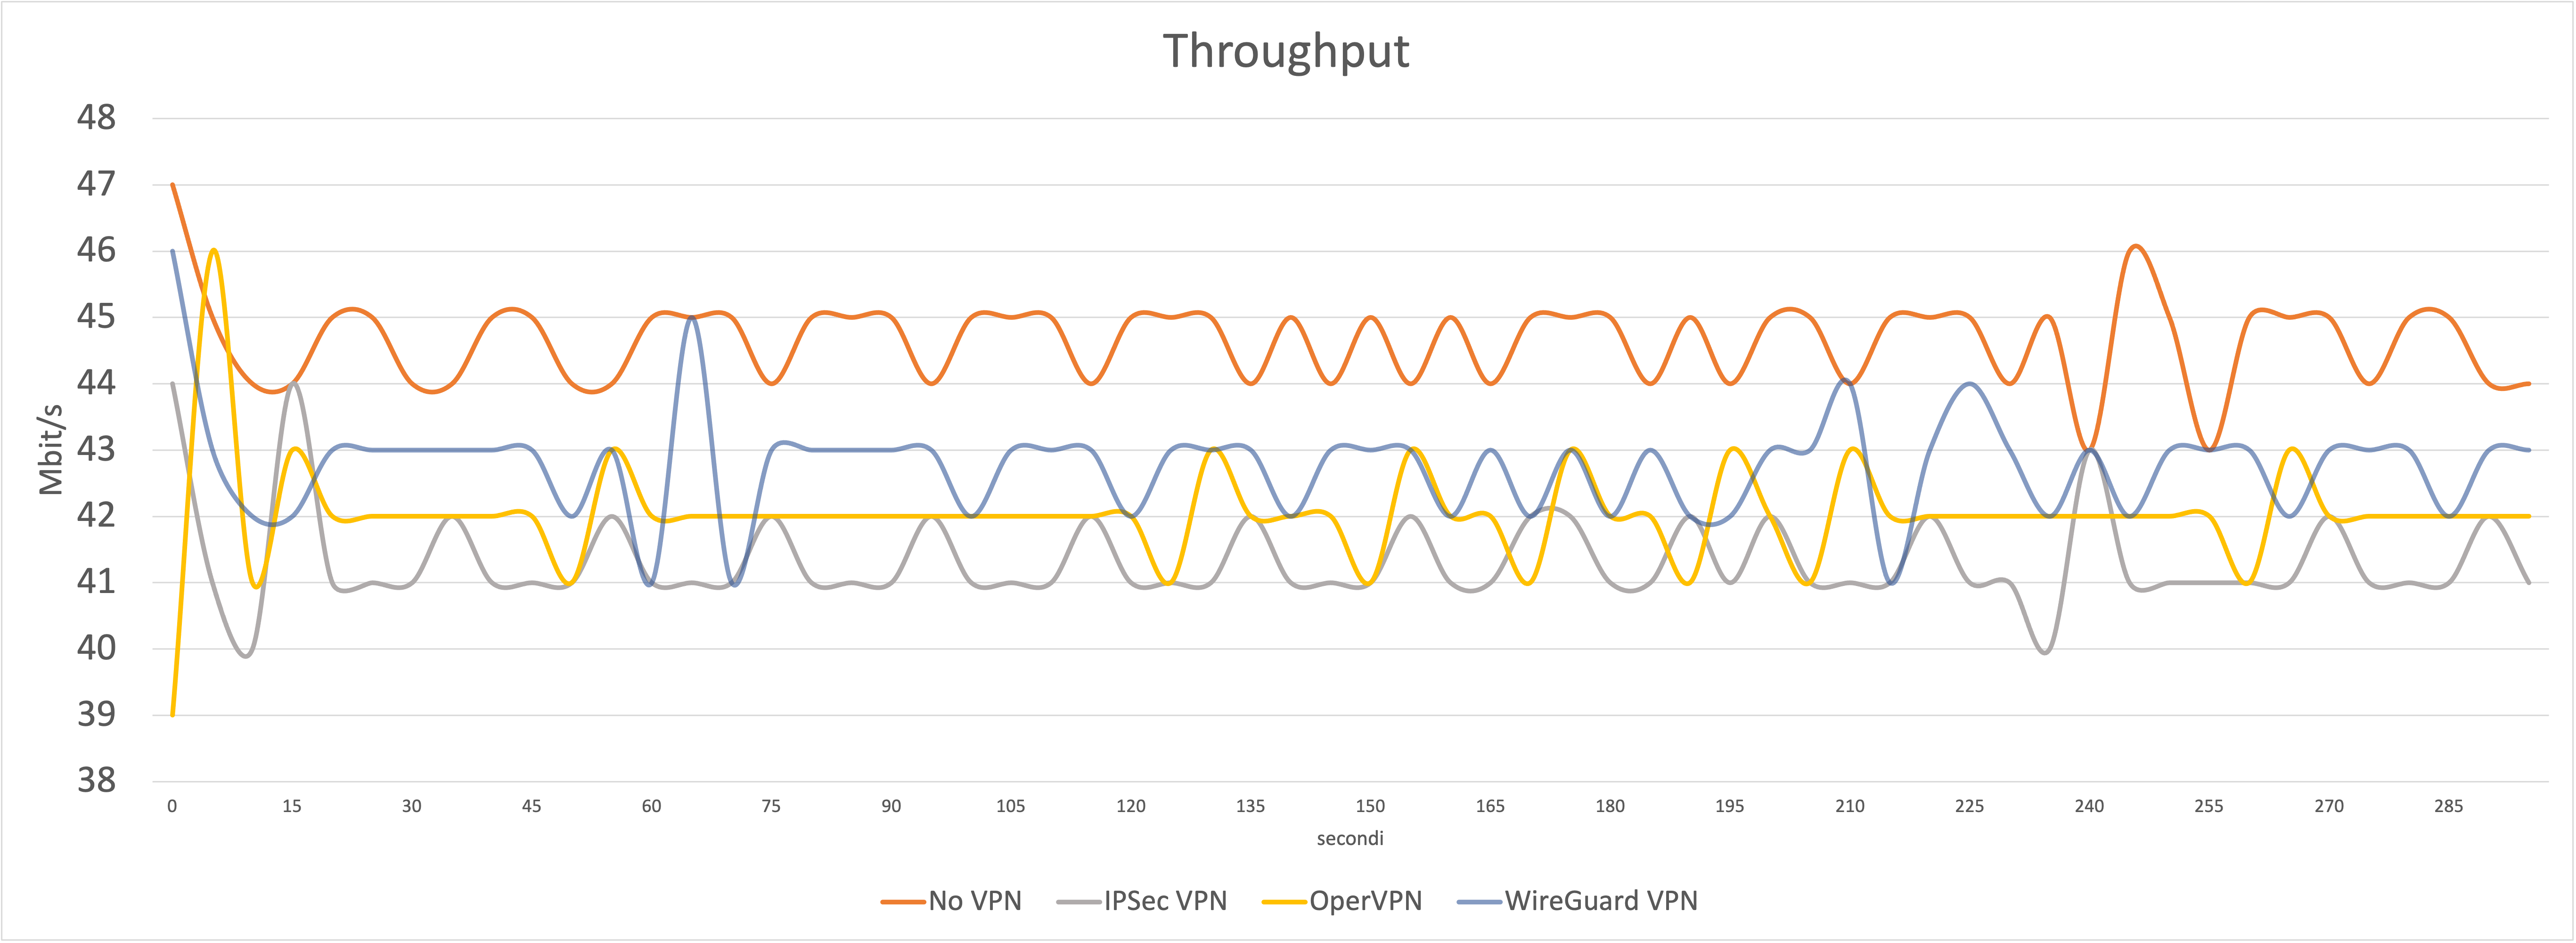
\includegraphics[width=14cm]{figure/fineThroughput.png}
    \caption{Confronto dei throughput raffinati}
\end{figure}

\begin{figure}[ht]
    \centering
    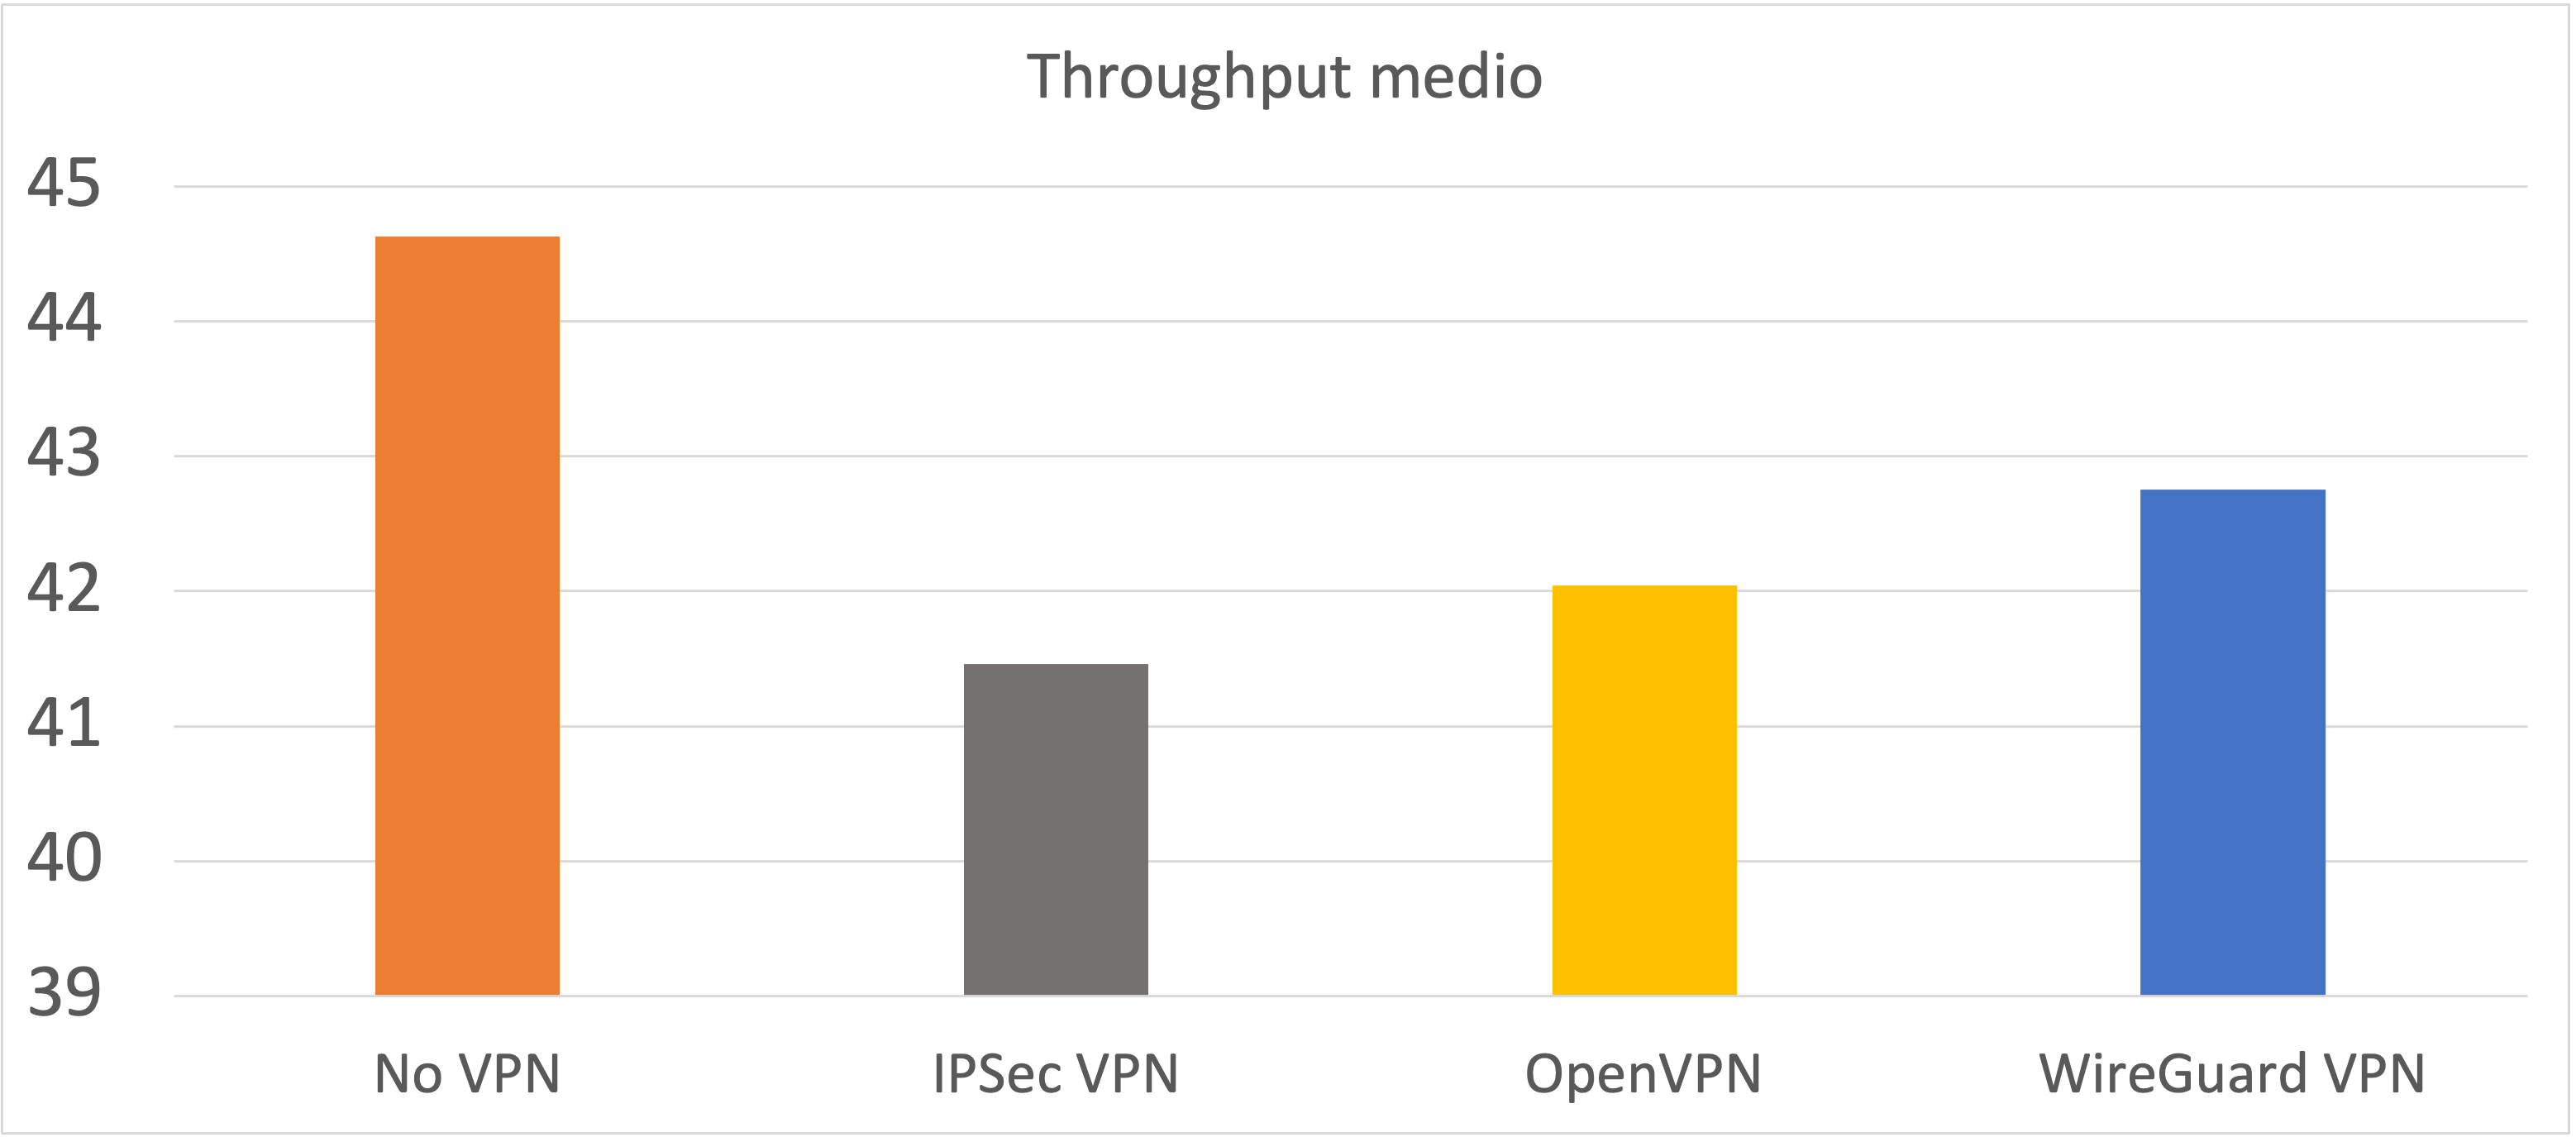
\includegraphics[width=10cm]{figure/avg.png}
    \caption{Confronto dei throughput medi}
\end{figure}